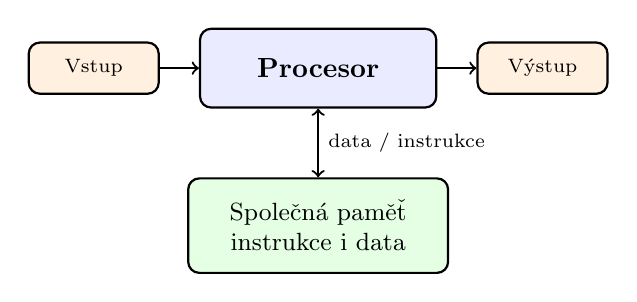
\begin{tikzpicture}[
    x=1cm, y=1cm,
    every node/.style={font=\small},
    unit/.style={
        draw,
        thick,
        rounded corners,
        align=center,
        minimum width=2.55cm,
        minimum height=0.80cm
    },
    subunit/.style={
        draw,
        rounded corners,
        align=center,
        fill=black!5,
        minimum width=2.25cm,
        minimum height=0.43cm,
        font=\scriptsize
    },
    arr/.style={->, thick},
    barr/.style={<->, thick}
]

    % CPU
    \node[
        unit,
        fill=blue!8,
        minimum width=3.00cm,
        minimum height=1.00cm,
        font=\bfseries
    ] (cpu) at (0,0) {Procesor};

    % Memory
    \node[
        unit,
        fill=green!10,
        minimum width=3.30cm,
        minimum height=1.20cm
    ] (memory) at (0,-2.00) {Společná paměť\\ instrukce i data};

    % I/O
    \node[
        unit,
        fill=orange!12,
        minimum width=1.65cm,
        minimum height=0.65cm,
        font=\scriptsize
    ] (inputnode) at (-2.85,0) {Vstup};

    \node[
        unit,
        fill=orange!12,
        minimum width=1.65cm,
        minimum height=0.65cm,
        font=\scriptsize
    ] (outputnode) at (2.85,0) {Výstup};

    % Arrows
    \draw[arr] (inputnode.east) -- (cpu.west);
    \draw[arr] (cpu.east) -- (outputnode.west);

    \draw[barr] (cpu.south) -- node[right, font=\scriptsize] {
        data / instrukce
    } (memory.north);

\end{tikzpicture}
